        %----------------------------------------------------------------------------------------
    %	PACKAGES AND THEMES
    %----------------------------------------------------------------------------------------
    \documentclass[aspectratio=169,xcolor=dvipsnames]{beamer}
    
    \usetheme{Boadilla}
    \usecolortheme{dolphin}
    
    \usepackage{tikz}
    \usetikzlibrary{arrows.meta}
    \usepackage{kbordermatrix}
    \usepackage[skip=2pt]{caption}
    \usepackage{algorithm, algorithmic}
    
    %----------------------------------------------------------------------------------------
    %	TITLE PAGE
    %----------------------------------------------------------------------------------------
    
    \title[Algorithms for Combinatorial Auction]{Algorithms for Combinatorial Auction} %\subtitle{}
    \author[Andrea Teruzzi] {Andrea Teruzzi}
    \date[20602 - Computer Science (Algorithms)]{May 26, 2022} 
    
    %----------------------------------------------------------------------------------------
    %	PRESENTATION SLIDES
    %----------------------------------------------------------------------------------------
    
    \begin{document}
    
    \begin{frame}
        % Print the title page as the first slide
        \titlepage
    \end{frame}
    %----------------------------------------------------
     \begin{frame}{Table of Contents}
        % Print the title page as the first slide
        \tableofcontents
    \end{frame}
    
    
    \AtBeginSubsection[]
    {
      \begin{frame}
        \frametitle{Table of Contents}
        \tableofcontents[currentsection,hideothersubsections,currentsubsection]
      \end{frame}
    }
    
    


    %------------------------------------------------
    \section{Combinatorial Auction Problem}
    %------------------------------------------------
    \subsection{Problem Statement }
    \begin{frame}{Problem Statement }
    \begin{block}{Combinatorial Auction Problem (CAP), \cite{algo_gt_nisan_ch11}}
    Let $\boldsymbol{M}$, with $|M| = m $, a set of items to be sold to $n$ bidders. Then we define
    $$
    \boldsymbol{v_i}: S \subseteq M\rightarrow v_i(S) \in \mathbb{R}
    $$
    
    as the \textbf{valuation} function for the i-th bidder, defined for each bundle of items $S$.\\
\pause
    Two common assumptions on $v_i$:
    \begin{enumerate}
        \item $v_i(\varnothing) = 0$ (\textbf{Normalized})
        \item $ S \subseteq T \subseteq M \Rightarrow v_i(S) \leq v_i(T) $
        (\textbf{Monotone})
    \end{enumerate}
\pause
    The objective of the problem is to find an \textit{allocation} $S_1 \cdots S_n$ with $S_i \cap S_j = \varnothing$  for every $ i \neq j$  that maximize the \textbf{common welfare}, namely:
    $$
    \max_{\substack{S_1 \cdots S_n}} \sum_{i} v_i(S_i) 
    $$
    \end{block}
    \end{frame}

   %------------------------------------------------
    \begin{frame}{Main problems for CAP}
    Examples of CAP problems:
    \begin{itemize}
        \item \textit{Spectrum auctions}
        \item \textit{Land Auctions}
        \item \textit{Logistic optimization}
    \end{itemize}
\pause
    \vspace{8pt}
    The main issues of the problem that we need to take care of are:
    \begin{enumerate}
        \item The optimization problem could be \textbf{computationally hard}.
        \item The input size is exponential, indeed each evaluation function $v_i$ requires $2^m$ estimates to be well defined, it is a \textbf{combinatorial problem}.
\pause
        \item How to \textbf{design an efficient auction}?
        \item How to take into account the \textbf{strategic behaviour} of bidders?
    \end{enumerate}
    \end{frame}
    
    %------------------------------------------------
    \subsection{Single-Minded Case}
    \begin{frame}{Single-Minded Case}
    Let us consider a \textbf{simplification of the CAP}, in particular we impose a restriction on the valuation functions:
    \begin{block}{Definition}
    We say a \textit{valuation} $v$ to be \textbf{single minded} if there exists a bundle of items $S^*$ and a value $v^* \in \mathbb{R}$ s.t.:
    $$
        v(S)= 
    \begin{cases}
        v^* & \text{if } S\supseteq S^* \\
        0              & \text{otherwise}
    \end{cases}
    $$
    \end{block}
    \vspace{8pt}
\pause
    Single minded valuations are very simply represented and the algorithmic allocation problem is given by:\\ \vspace{3pt}
    \textbf{INPUT: } $(S^*_i, v^*_i)$ for each bidders $ i = 1 \cdots n$ \\
    \textbf{OUTPUT: } A winner subset $\boldsymbol{W} \subseteq \{1, \cdots ,n\}$ such that $S_i \cap S_j = \varnothing$ for every  $i \neq j$
    \end{frame}
    
    
    %------------------------------------------------
    \begin{frame}{Single-Minded Case – NP-hardness}
    \begin{block}{Proposition}
    The allocation problem among single-minded bidders is \textbf{NP-Hard}
    \end{block}
\pause
    \textbf{Proof}\\
    Consider the \textbf{Independent Set Problem} (\textbf{ISP}), namely given a graph $\mathcal{G} = (\mathcal{E},\mathcal{V})$ find the largest possible independent set. This problem is known to be NP-hard.\\
\pause
    Then consider the following graph $G = (E,V)$:
    \begin{itemize}
        \item The set of edges $E$ to be the set of items.
        \item The set of vertexes $V$ to be the bidders. For vertex $i \in V$, we will have the desired bundle of $i$ to be the set of adjacent vertices, namely $S^*_i = \{e \in E : i \in e\}$ and the value will be $v^*_i = 1$.
    \end{itemize}
\pause
    Now notice that a set $W$ of winner in the CAP problem satisfies $S^*_j \cap S^*_i = \varnothing$ for every $i \neq j \in W$ if and only if the set of vertices is an independent set in $G$. The social welfare of $W$ is exactly the size of the independent set in $G$. \hspace{1pt} $\Box$ 
    
    
    %------------------------------------------------
    \end{frame}
    \begin{frame}{Single-Minded Case – Example}
    \begin{figure}
    \setlength{\abovecaptionskip}{20pt}
    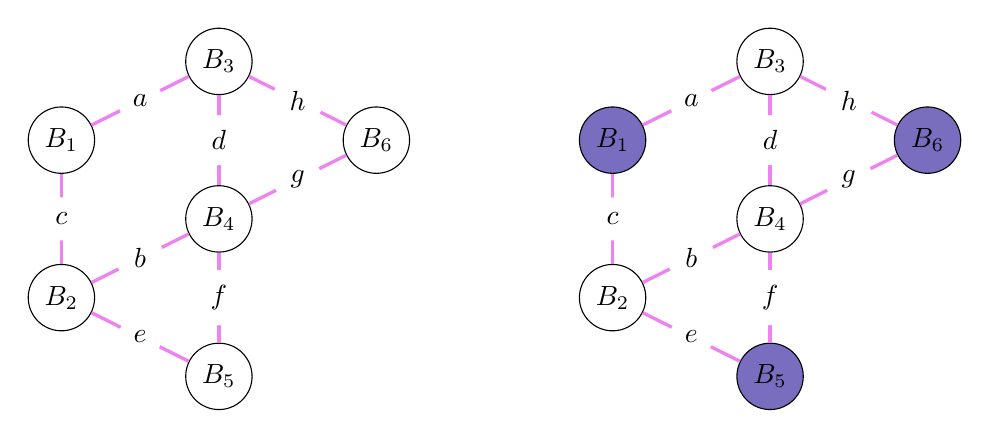
\begin{tikzpicture}[scale = 1]
    \begin{scope}[every node/.style={circle,draw}]
        \node (A) at (3, 1.2) {$B_2$} ;
        \node (B) at (3, 3.2) {$B_1$} ;
        \node (C) at (5, 4.2) {$B_3$};
        \node (D) at (5, 2.2) {$B_4$} ;
        \node (E) at (5, 0.2) {$B_5$};
        \node (F) at (7, 3.2) {$B_6$} ;

       \uncover<2->{ \node (A2) at (11 - 1, 1.2) {$B_2$};
        \node[fill = Periwinkle] (B2) at (11 - 1,2+1.2) {$B_1$} ;
        \node (C2) at (13 - 1, 3+1.2) {$B_3$};
        \node (D2) at (13 - 1,1+1.2) {$B_4$} ;
        \node[fill = Periwinkle] (E2) at (13 - 1, 0.2) {$B_5$};
        \node[fill = Periwinkle] (F2) at (15 - 1, 3.2) {$B_6$} ;}
       
        
    \end{scope}
    \begin{scope}[>={Stealth[black]},
                  every node/.style={fill=white,circle},
                  every edge/.style={draw = Violet, very thick}]
        \path (B) edge node {$a$} (C);
        \path (A) edge node {$b$} (D);
        \path (A) edge node {$c$} (B);
        \path (D) edge node {$d$} (C);
        \path (A) edge node {$e$} (E);
        \path (D) edge node {$f$} (E);
        \path (D) edge node {$g$} (F);
        \path (C) edge node {$h$} (F);
        
       \uncover<2->{ \path (B2) edge node {$a$} (C2);
        \path (A2) edge node {$b$} (D2);
        \path (A2) edge node {$c$} (B2);
        \path (D2) edge node {$d$} (C2);
        \path (A2) edge node {$e$} (E2);
        \path (D2) edge node {$f$} (E2);
        \path (D2) edge node {$g$} (F2);
        \path (C2) edge node {$h$} (F2);}
    
    \end{scope}
    \end{tikzpicture}
    \caption{Example of CAP adapted to ISP} \label{fig:1}
    \end{figure}
    \end{frame}
    

    %------------------------------------------------
    \subsection{Bidding Languages}
    \begin{frame}{Bidding Languages}
    With respect to the problem of representing bidders valuations, we have to consider the following problems:
        \begin{itemize}
        \item A naive approach asking for a valuation for each set would require a real value for each $\mathbf{2^m -1}$ \textbf{non-empty set} for each bidder, which could be computationally unmanageable even with few items.
        \item We are looking for \textbf{bidding languages} that allow bidders to encode \textbf{succinctly} and  \textbf{effectively} their valuations and send them to the auctioneer. 
        \item In designing bidding languages we face an \textbf{expressiveness–simplicity tradeoff}.
    \end{itemize}
\pause
    Commonly used bidding languages are:
            \begin{enumerate}
                \item \textbf{OR bid}
                \item \textbf{XOR bid}
                \item \textbf{OR/XOR bid}
            \end{enumerate}
    \end{frame}
    
    %----------------------------
    \begin{frame}{Bidding Languages – OR bids}
    Common bidding languages are combinations of \textbf{atomic bids}. This simple evaluations are in the form $\boldsymbol{(S,p)}$, meaning an offer of $p$ monetary units for any bundle $T$, with $T \supseteq S$.
\pause
    \begin{block}{OR bids}
    \textbf{OR language} considers different bids as totally independent. Given an OR valuation for the $j-th$ bidder $v_{j} = (S_1, p_{1})OR \dotsc OR  (S_k, p_{k})$, the valuation for the bundle $S$ is:  
    $$
    v(S) = \max_{W} \sum_{j \in W} p_i
    $$
    where $W$ is valid collection of pairs, meaning for all $i \neq j \in W, S_i \cap S_j = \varnothing$. \\
    \smallskip
\pause
    OR can represent only \textbf{superadditive} valuations, namely:
    $$
     v(S \cup T) \geq v(S) + v(T) \quad \forall S \cap T = \varnothing
    $$
    \end{block}
    \end{frame}
    
    %----------------------------
    \begin{frame}{Bidding Languages}
    
    \begin{block}{XOR bids}
    \textbf{XOR language} considers different bids as totally mutually exclusive. Given a XOR valuation for the $j-th$ bidder $v_j = (S_1,p_{1})XOR  \dotsc XOR  (S_k,p_{k})$, the valuation for the bundle $S$ is:  
    $$
    v_j (S) = \max_{\substack{i | S_i \subseteq S_n}} p_i
    $$
\pause
    XOR can directly represent \textbf{unit demand} valuations of this kind:
    $$
    v (S) = \max_{\substack{j \in S}} v(\{p_i\})
    $$
    and thus it can represent \textbf{every valuations}, but with bids of \textbf{exponential size}!
\pause
    \end{block}
    It is possible to form general combinations of \textbf{OR/XOR}:
    \begin{align*}
       \boldsymbol{e.g.} \hspace{5pt}  v(S) &= (u)OR (\{d\},5)\\
                               \uncover<2->{&= \big( (\{a,b\},3)XOR (\{c\},2) \big)OR (\{d\},5)}
    \end{align*}
    \end{frame}
    
    %----------------------------
    \begin{frame}{Bidding Languages – Example}
    \vspace{-30pt}
    \begin{align*}
      \boldsymbol{e.g.}  \hspace{4pt} & v(S) = (\{a,b\},3)OR(\{c,d\},5)   &&u(S) = (\{a,b\},3)XOR(\{c,d\},5) \\
                        \uncover<2->{& v(\{a,c\}) = 0 &&u(\{a,c\}) = 0} \\
                        \uncover<3->{& v(\{a,b\}) = 3 &&u(\{a,b\}) = 3} \\
                        \uncover<4->{& v(\{a,b,c,d\}) = 8 && u(\{a,b,c,d\})=5} \\
                          & \\
                        \uncover<5->{& w(S)= (\{a,b,\boldsymbol{D_{1}}\},3)OR(\{c,d,\boldsymbol{D_{1}}\},5)}\\
                        \uncover<6->{& w(\{a,c\}) = 0 }\\
                        \uncover<7->{& w(\{a,b\}) = 3 }\\
                        \uncover<8->{& w(\{a,b,c,d\}) = \mathbf{5}}
    \end{align*}

    \uncover<9->{We call this formulation $\mathbf{OR^*}$, defined on $M \cup D$, with $D$ adequate set of dummy variables.}
    \end{frame}
    
    %-------------------------------------
    \begin{frame}{Bidding Languages – Closing words}

    \textbf{OR} bids can represent \textbf{only superadditive valuations}, while \textbf{XOR} can represents \textbf{every valuation}, however for additive evaluations they need a \textbf{bid of exponential size}.
\pause
    \begin{block}{Proposition}
    Any valuation OR/XOR of size s can be represented by $OR^*$ bids of size s using at most $s^2$ dummy items.
    \end{block}
\pause
    $OR^*$ is a very appealing bidding language:
    \begin{itemize}
    \item $OR^*$ bids look like a regular OR on a larger set of items.
\pause
    \item $OR$ looks at an allocation algorithm just like a collection of \textbf{atomic bids from different players}. We can use the \textbf{same algorithms for single-minded bids} (it does not matter the number of bidders).
    \end{itemize}

\end{frame}



   %-------------------------------------------------
    \section{Algorithms for solving CAP}
    \subsection{Integer programming formulation of CAP}
    \begin{frame}{Integer programming formulation of CAP}
        \begin{block}{CAP ILP, \cite{cap_survey}}
        Let $N$ be the set of n bidders and $M$ the set of $m$ items. For every subset $S \subseteq M$ let $b_j(S)$ be the bid of the agent $j \in N$ for $S$. Let $b(S)= \max_{j \in N}b_j(S)$ and $x_S = 1$ when the set $S$ is accepted, while $x_S = 0$ when the  set is refused.\\
\pause
        Then the CAP problem can formulated as the following integer program:
        \begin{gather*}
            \max \sum _{S\subset M} b(S)x_S \\
            s.t. \hspace{8pt} \sum _{S \ni i} x_S \leq 1 \hspace{8pt} \forall i \in M \\ 
            x_S \in \{0,1\} \hspace{8pt} \forall S\subset M
        \end{gather*}
        \end{block}
    \end{frame}
     %-------------------------------------------------
     \begin{frame}{Integer programming formulation of CAP}
     $\boldsymbol{OR^*}$ bids give the possibility to \textbf{express general problems in term of atomic bids} as in the single minded case. \\
\pause
     Consider this \textbf{example}:
     \vspace{-10pt}
   
    \begin{flalign*}
   \mathbf{x} &= \left[\begin{array}{ccccc}x_{\{a\}} & x_{\{b\}} & x_{\{c\}} & x_{\{a,b\}} & x_{\{a,b,c\}}\end{array}\right]^\intercal \\
    \mathbf{b} &= \left[\begin{array}{ccccc}\max_{j \in N}b_j\{a\} & \max_{j \in N}b_j{\{b\}} & \max_{j \in N}b_j{\{c\}} & \max_{j \in N}b_j{\{a,b\}} & \max_{j \in N}b_j{\{a,b,c\}} \end{array}\right]^\intercal 
    \end{flalign*}
    
    \vspace{-10pt}
    \begin{columns}[t]
    \uncover<3->{\begin{column}{0.45\linewidth}
    \[
    \mathbf{A} = \kbordermatrix{
    & \{a\} & \{b\} & \{c\} & \{a,b\} & \{a,b,c\} \\
    a & 1 & 0 & 0 & 1 & 1 \\
    b & 0 & 1 & 0 & 1 & 1 \\
    c & 0 & 0 & 1 & 0 & 1 
    }
    \]
    \end{column}}
    \uncover<4->{
    \begin{column}{0.55\linewidth}
    \begin{gather*}
       \max \mathbf{b}^\intercal \mathbf{x}  \\
        \text{s.t} \quad \mathbf{A}\mathbf{x} \leq \mathbf{1} \\ 
        x_{i} \in \{0,1\} \hspace{4pt} \forall i
     \end{gather*}
    \end{column}}
    \end{columns} 
     
     
     
     \end{frame}
    %------------------------------------------------
    \begin{frame}{Integer programming}
    The \textbf{integer programming} is known to be \textbf{NP-hard}. However, in literature there are known several ways to tackle this problem : 
\pause
    \begin{enumerate}
        \item \textbf{Solvable instances} 
            \begin{itemize}
            \item \textit{Totally unimodular matrix}
            \item \textit{Balanced matrix}
            \end{itemize}
\pause
        \item \textbf{Approximations}
         \begin{itemize}
            \item \textit{Worst case analysis}
            \item \textit{Probabilistic analysis}
            \end{itemize}
\pause
        \item \textbf{Exact methods}
         \begin{itemize}
            \item \textit{Branch and bound}
            \item \textit{Cutting planes}
            \item \textit{Branch and cut}
            \end{itemize}
    \end{enumerate}    
\pause
    The \textbf{combinatorial nature} of the problem, combined with the fact that general instances of the problem are \textbf{not polynomial} leads to a \textbf{very hard framework}(e.g. $2^{20} \approx 10^6$ columns).
    \end{frame}
    
    %------------------------------------------------
    \subsection{Greedy Mechanism for Single-Minded Bidders}
    \begin{frame}{Approximation Single-Minded Bidders}
    
    \begin{algorithm}[H]
    \begin{algorithmic}[1]
    \REQUIRE Ordered set of single minded bids such that $\frac{v^{*}_{1}}{\sqrt{|S^{*}_{1}|}} \geq \frac{v^{*}_{2}}{\sqrt{|S^{*}_{2}|}} \geq \cdots \geq \frac{v^{*}_{n}}{\sqrt{|S^{*}_{n}|}}  $
    \uncover<2->{\STATE $W \leftarrow \varnothing $
    \FOR{$i=1$ to $N$}
    \IF {$S^{*}_{i} \cap \Big(\bigcup_{j \in W} S^{*}_{j} \Big) = \varnothing$}
    \STATE $W \leftarrow W \cup {i}     $
    \ENDIF
    \ENDFOR}
    \uncover<3->{\ENSURE The set of winners $W$.}
    \end{algorithmic}
    \caption{Greedy Mechanism for Single-Minded Bidders}
    \label{alg:seq}
    \end{algorithm}
    \vspace{-10pt}
    \begin{itemize}
       \uncover<4->{ \item Using $OR^*$ as bidding language, we can apply this algorithm to the CAP in ILP form and not only to Single-Minded Bidders ($i.e. \hspace{2pt} |S^{*}_{j}|= \sum_{i \in m}aij $).}
        \uncover<5->{\item It is \textbf{efficiently computable} in polynomial time.} 
        %The time complexity is dominated by the  sorting operation, which is $O(n \log n)$.
    \end{itemize}
    
    \end{frame}
    
     %------------------------------------------------
    \begin{frame}{Greedy Mechanism for Single-Minded Bidders }
    \begin{block}{Proposition}
    The Greedy mechanism for Single-Minded Bidders \textbf{achieves a $\sqrt{m}$ approximation}. \uncover<2->{Namely, for the allocation $OPT$ with the maximum value of $\sum_{j \in OPT} v^{*}_{j}$:
    $$
    \sum_{j \in OPT} v^{*}_{j} \leq \sqrt{m} \sum_{j \in W} v^{*}_{i}
    $$
    with $W$ the output of the greedy algorithm.}
    \end{block}

    \uncover<3->{\textbf{Proof} \\
    For each $i \in W$ let $OPT_{i}= \{ j \in OPT, j \geq i | S^{*}_{i} \cap S^{*}_{j}  \neq \varnothing \}$.} \uncover<4->{Then $OPT \subseteq \bigcup_{i \in W} OPT_{i} $ and thus it is enough to prove: }
    
    \uncover<4->{
    $$\forall i \in W, \sum_{j \in OPT_{i}} v^{*}_{j} \leq \sqrt{m} v^{*}_{i}$$}
    \end{frame}
    
    %------------------------------------------------
    \begin{frame}{Greedy Mechanism for Single-Minded Bidders II}
    Note for every $j \in OPT_i$  $v^{*}_{j} \leq \frac{v^{*}_{i} \sqrt{|S^{*}_{j}|}  }{\sqrt{|S^{*}_{i}|}}$. Then, we can sum over all $j \in OPT_{i}$:
    \begin{equation}
    \sum_{j \in OPT_{i}}v^{*}_{j} \leq \frac{v^{*}_{i} }{\sqrt{|S^{*}_{i}|}} \sum_{j \in OPT_{i}} \sqrt{|S^{*}_{j}|}
    \end{equation}
\pause
    Using the Cauchy-Schwarz inequality we can bound the second member of the RHS of (1):
    \begin{align*}
        \sum_{j \in OPT_{i}} \sqrt{|S^{*}_{j}|}\cdot 1 &\leq \sqrt{\sum_{j \in OPT_{i}}1} \sqrt{\sum_{j \in OPT_{i}}|S^{*}_{j}| }\\
          &= \sqrt{| OPT_{i}|} \sqrt{\sum_{j \in OPT_{i}}|S^{*}_{j}| }
    \end{align*}
    \end{frame}
    
     %------------------------------------------------
    \begin{frame}{Greedy Mechanism for Single-Minded Bidders III}
    From the definition of $OPT_{i}$ it follows $|OPT_{i}| \leq |S^{*}_{i}|$ and since OPT is an allocation $\sqrt{\sum_{j \in OPT_{i}} |S^{*}_{j}|} \leq \sqrt{m}$. 
    \pause We can substitute these two results in the Cauchy-Schwarz inequality obtaining:
    \vspace{-5pt}
    \begin{align*}
        \sum_{j \in OPT_{i}} \sqrt{|S^{*}_{j}|} &\leq \sqrt{| OPT_{i}|} \sqrt{\sum_{j \in OPT_{i}}|S^{*}_{j}| }\\
                                                &\leq \sqrt{|S^{*}_{i}|}\sqrt{m}
    \end{align*}
    
\pause
    Plugging this result in (1) we obtain:
    \vspace{-5pt}
    \begin{align*}
    \sum_{j \in OPT_{i}}v^{*}_{j} &\leq \frac{v^{*}_{i} }{\sqrt{|S^{*}_{i}|}} \sum_{j \in OPT_{i}} \sqrt{|S^{*}_{j}|} \\
                                  &\leq  \sqrt{m} v^{*}_{i} \hspace{6pt} \Box 
    \end{align*}
    
    \end{frame}
     
     %------------------------------------------------
     \begin{frame}{Greedy Mechanism for Single-Minded Bidders}
     \begin{figure}
        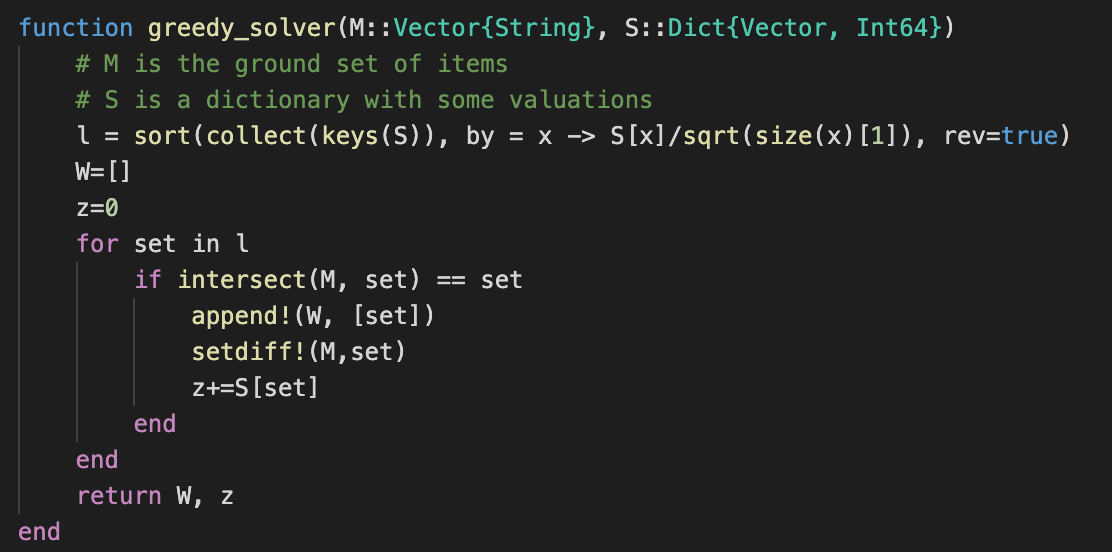
\includegraphics[width=1\textwidth, height=0.7\textheight, keepaspectratio]{utilities/greedy.png}
        \caption{Greedy algorithm in Julia} \label{fig:2}
    \end{figure}
     
     \end{frame}
     %------------------------------------------------
    \subsection{Solving Integer Programs in Julia}
    \begin{frame}{Exact Solutions for ILP}
    For obtaining exact solutions (or at least better approximations) we need more involved algorithms, mainly based on the simplex algorithm.  
    \vspace{10pt}
\pause
    \begin{itemize}
        \item \textbf{JuMP} is package in \textbf{Julia} used for solving optimization program. It uses algebraic modeling languages, such as \textbf{HiGHS} for designing and solving efficiently LP and ILP.
\pause        
        \item For solving LP it uses a parallelized version of the  \textbf{revised dual simplex} algorithm.
\pause
        \item It uses branch and bound algorithms to solve ILP when there are few columns.
\pause
        \item Some applications can be found at \url{https://github.com/andreateruzzi/combinatorial_auction_ILP}.
    \end{itemize}
 
    \end{frame}
    %------------------------------------------------
     \begin{frame}{Exact Solutions for ILP}
     \begin{figure}
        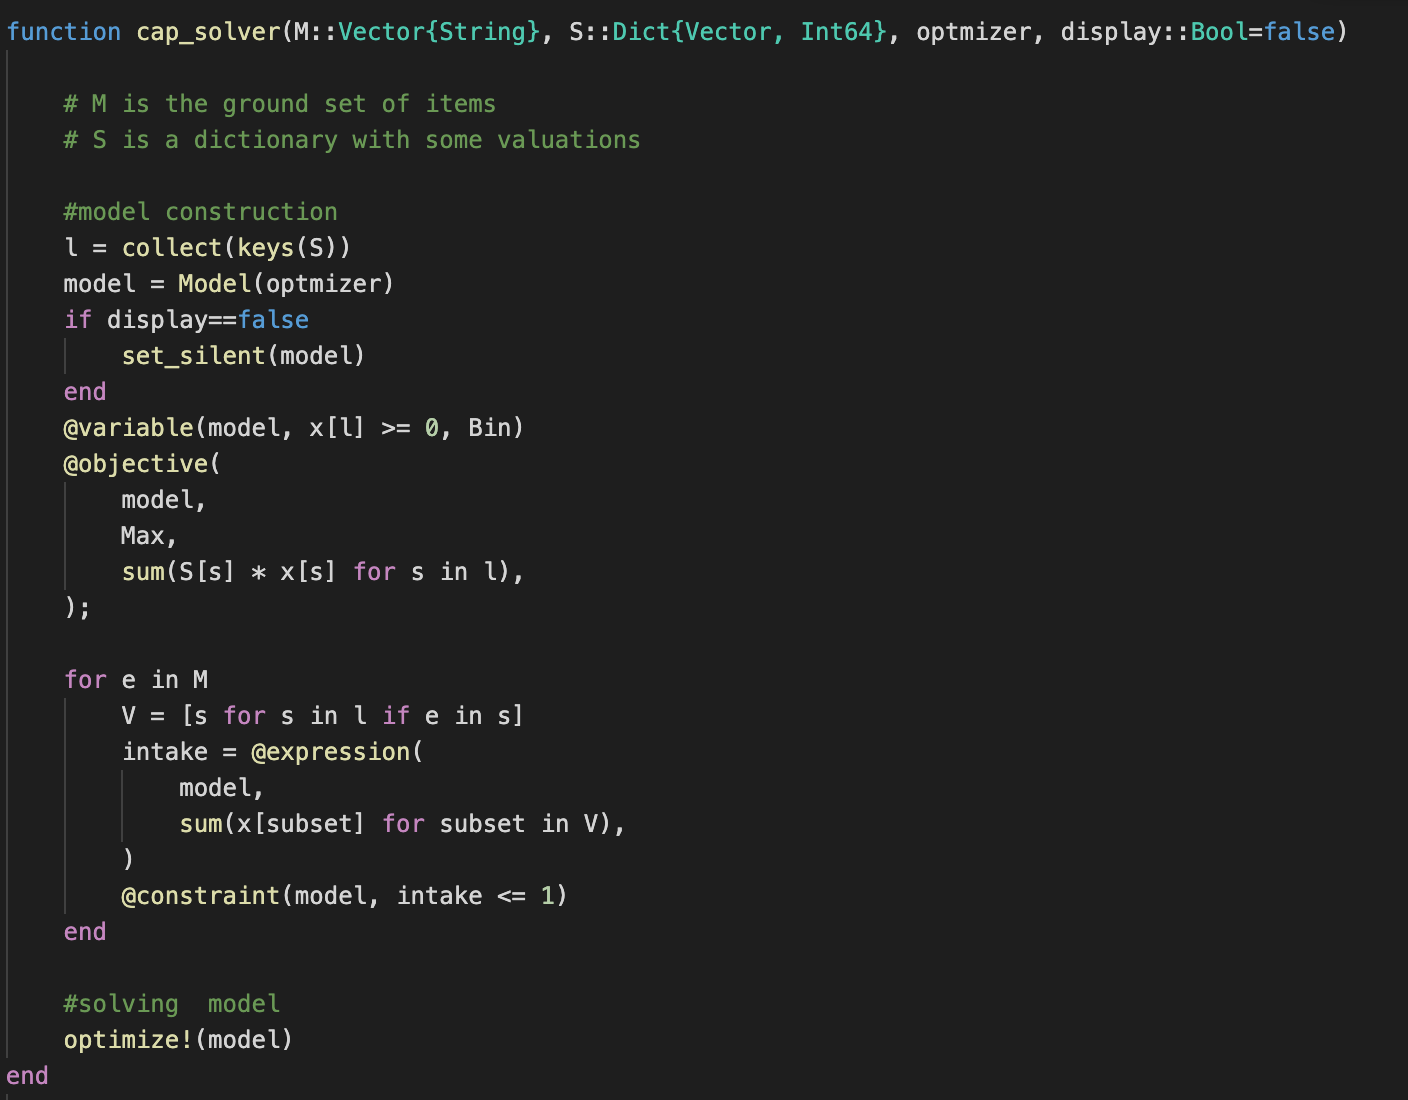
\includegraphics[width=1\textwidth, height=0.7\textheight, keepaspectratio]{utilities/cap_solver.png}
        \caption{Integer program solver in Julia} \label{fig:3}
    \end{figure}
     
     \end{frame}
    %-------------------------------------------------------
    \begin{frame}{Exact Solutions for ILP – Example}
    \vspace{-15pt}
    \begin{flalign*}
    \text{\textbf{INPUT}: } \mathbf{M} =\{a,b,c\} \uncover<2->{&\rightarrow v_{1} = (\{a\},3)OR(\{b\},3)OR(\{c\},3) && \\
                                      &\rightarrow v_{2} = (\{a,b\},5)OR(\{b\},4)OR(\{a,b,c\},6) && \\ &\rightarrow v_{3} = (\{c\},5)  &&}
    \end{flalign*}
    \vspace{-30pt}
    \begin{columns}[t]
    \begin{column}{0.48\linewidth}
    \begin{flalign*}
    \uncover<3->{\mathbf{x} &= \left[\begin{array}{ccccc}x_{\{a\}} & x_{\{b\}} & x_{\{c\}} & x_{\{a,b\}} & x_{\{a,b,c\}}\end{array}\right]^\intercal \\
    \mathbf{b} &= \left[\begin{array}{ccccc}3 & 4 & 5 & 5 & 6 \end{array}\right]^\intercal  }
    \end{flalign*}
    \end{column}
    \begin{column}{0.55\linewidth}
     \uncover<4->{\[
    \mathbf{A} = \kbordermatrix{
    & \{a\} & \{b\} & \{c\} & \{a,b\} & \{a,b,c\} \\
    a & 1 & 0 & 0 & 1 & 1 \\
    b & 0 & 1 & 0 & 1 & 1 \\
    c & 0 & 0 & 1 & 0 & 1 
    }
    \]}
    \end{column}
    \end{columns} 
    
    
    \begin{gather*}
        \uncover<5->{\max z=\mathbf{b}^\intercal \mathbf{x}  \\
        \text{s.t } \quad \mathbf{A}\mathbf{x} \leq \mathbf{1} \\ 
        x_{i} \in \{0,1\} \hspace{4pt} \forall i }\\ 
         \uncover<6->{\text{\textbf{OUTPUT}: } \mathbf{x^{*}} = \left[\begin{array}{ccccc} 1 & 1 & 1 & 0 & 0 \end{array}\right]^\intercal\\
         z^* = 12 \hspace{25pt}}
     \end{gather*}
    
\pause
    \end{frame}
    
    

    %------------------------------------------------
    \begin{frame}[allowframebreaks]{Bibbliography}
    \bibliographystyle{alpha}
    \nocite{algo_gt_nisan_ch11, cap_survey, intro_algo, JuMP}
    \bibliography{bibl.bib}
        
    \end{frame}
    
    
    %----------------------------------------------------------------------------------------
    
    \end{document} 